
\documentclass{article}

\usepackage[utf8]{inputenc}
\usepackage[left=1.5in,right=1.5in,bottom=1in]{geometry}
 \usepackage{setspace} \onehalfspacing
\setlength\parindent{0pt}
\setlength{\parskip}{1em}
\setcounter{secnumdepth}{0}
\usepackage{outlines}
\usepackage{graphicx}
\usepackage{caption}
\graphicspath{ {imgs} }
\usepackage{hyperref}
\usepackage{enumerate}


\usepackage[
backend=biber,
style=alphabetic,
sorting=ynt
]{biblatex}
\addbibresource{photo_essay.bib}

\title{The Triangle of Ninoofsepoort}
\author{Carla Hyenne}

\begin{document}

\maketitle

\begin{figure}[h!]
	\centering
	\captionsetup{labelformat=empty}
	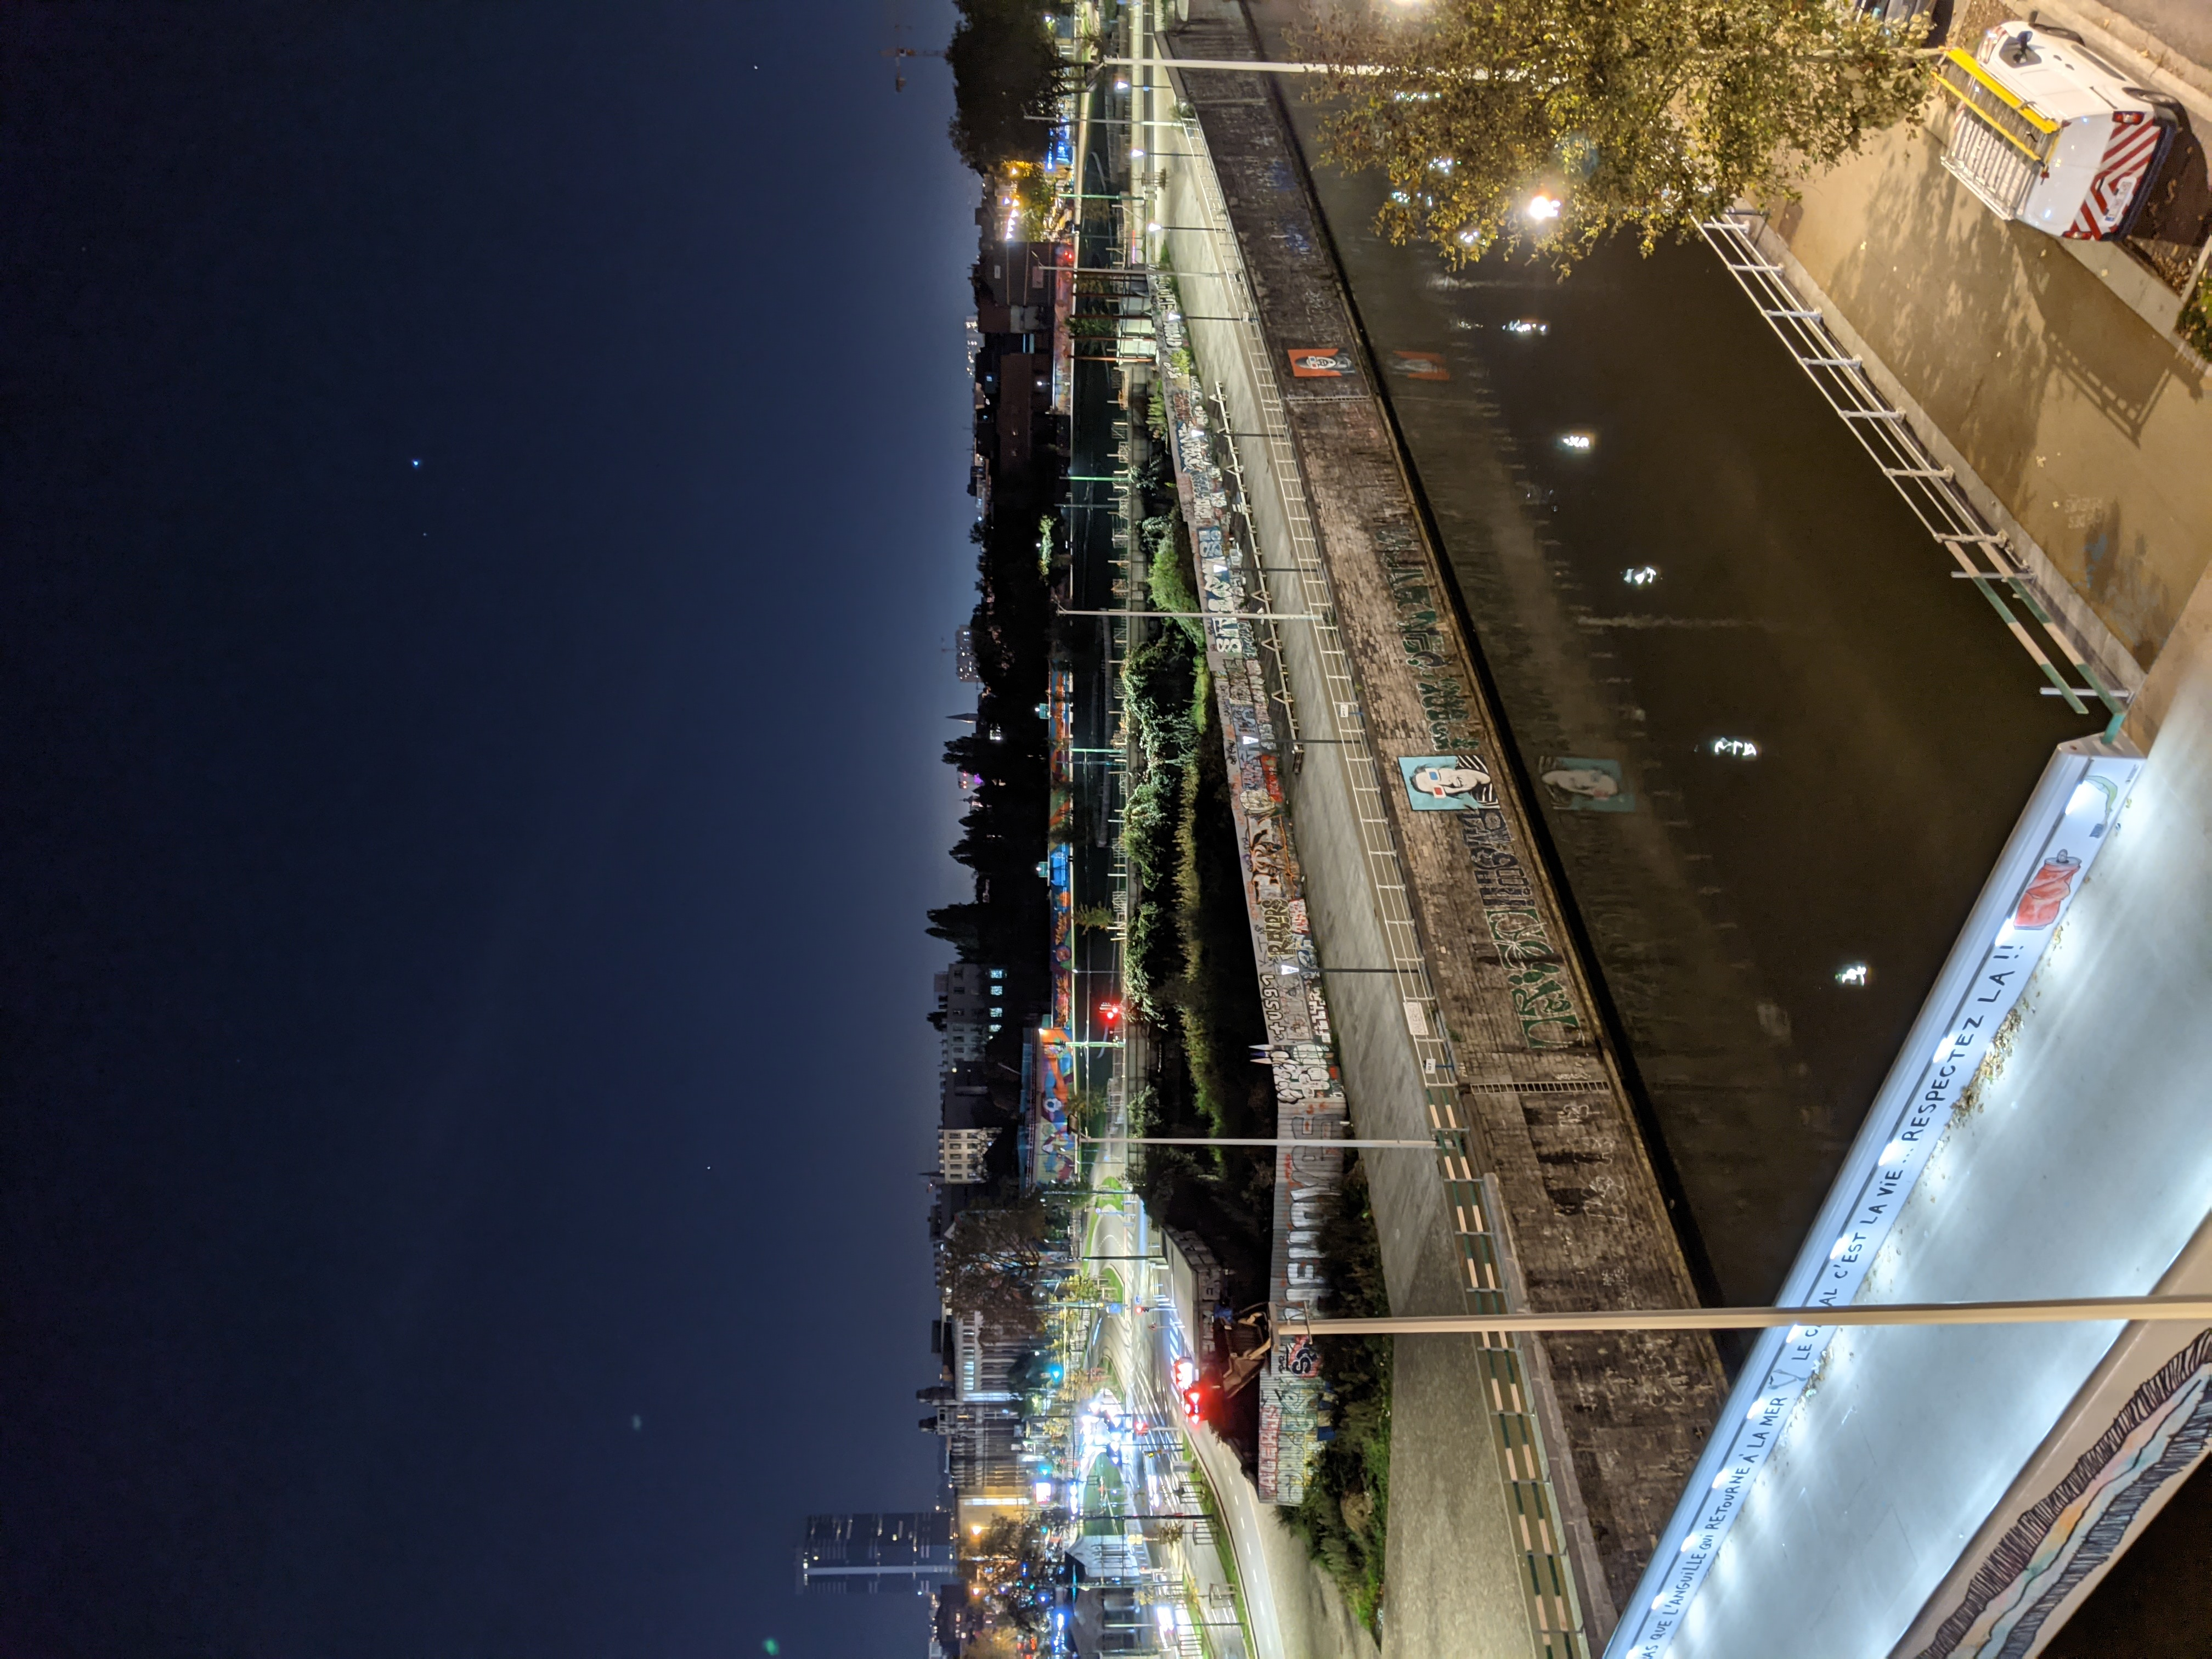
\includegraphics[width=\textwidth, angle=-90]{bxl_canal_far}
	\caption{View towards the Ninoofsepoort park from the rooftop of the MIMA museum, Sint-Jans-Molenbeek, October 23rd 2021}
\end{figure}

\pagebreak

%%%% History
Since mid-20th century, the Ninoofsepoort area was occupied by warehouses belonging to various companies including Bruxelles Proprete (Brussels Sanitation).

%%%% Ninoofsepoort Development
perspective.brussels was mandated by government in 2016 to develop Ninoofsepoor
Development site is located between west and east of Brussels, on the edge of the canal, at the border of the historical city centre, ``la petite ceinture''.
There was a large piece of land for development, on which the Ninoofsepoort park was developed. 
Now, there is a triangular area of land that remains unbuilt - what to do about it? The goal is ``véritable lieu de convivialité et d’attractivité pour toutes les populations'' \cite{perspectiveNinove}\marginpar{todo: translate}
Private investors and public authorities are involved.
The developers want the development to address not only local, but supra-local stakes

Parc de la Sennette, a project by the Contrat de Rénovation Urbaine ``Heyvaert-Poincaré''. Does this have to do with dislodging the Heyvaert street and businesses\marginpar{Creative and capitalist destruction}

Ninoofsepoort is part of the Canal Plan. As part of the plan, it fits has to respond to multiple criteria:\cite{diagnosticNinove}
- greenifying the area, with new park(s) and green belts
- the central bit of Ninoofseport is designated as a location for a potential high-rise build
- facilitating transport (public, private, cyclists, pedestrians)

%%%% The triangle
Privately owned, need to find out by whom, whereas the park area is owned by the Brussels-Capital region
Who is the owner though? It looks like its in a `zone administrative', which doesn't sound private

The plan is for three housing towers and `metropolitan equipment' 
Owned by Besix Red (need a bit more info on them)
It will have 270 private housing units, non of which will be social housing
The ground floor will be open, as to keep a cohesive urban fabric (they don't want a tower closed off to the outside)
It will have 240 parking spots, including 
Isn't this contradictory with the goal of facilitating a `soft' mode of transport? Why are they building these parking spots, do people in the area typically need these spots, or even have cars? It assumes that the people who will come to live in this towers are ones who need a car on a (semi) regular basis, perhaps to drive to work.
Even if the development of these housing towers is not directly destroying or displacing anyone, it contributes to slow process of gentrification in Moelenbeek. It indirectly raises the attractiveness of the area, thus rising prices, and displacing people and businesses who either cannot afford the new rent or are forced out for the urban regeneration cause. 

This development is also a stark contrast to the resident's demands for their neighbourhood, when they were consulted in 2014

Going beyond the photograph, the Canal Project continues towards Rue Heyvaert. The Contract de Quartier Durable project ``Petite Senne'' his displaces legal, second-hand car dealerships, which have been anchored in Rue Heyvart for centuries (?). 

Yet, we can't ignore that the triangle is inscribed within the entire Ninoofsepoort project, in which there is another project by the SLRB which will be 60\% social housing.


%%%% Stakes
The location is extremely attractive: between the West and Central train stations, on the canal, on the edge of the Pentagon, on two metro lines, and on the ``Petite Ceinture'', or the small ring, which surrounds the historical centre of Brussels. It's location on the canal means that the Ninoofsepoort is inscribed in the city's canal development plan.

Will the development match the goals envisioned by perspective.brussels?
What are these goals?
	- Anchor Ninoofsepoort in the small ring, and give it an identity, and improve urban space quality

%%%% Citizen Participation
Consultations citoyennes - citizen participation\marginpar{Lecture 5}

%%%% Conclusion
It hasn't been decided what will be built in the triangle, but we can imagine.

%%%%  From Urban Analysis
investing money in disadvantaged neighbourhoods, will accelerate gentrification, if there are no policies to reduce unemployment and improve living conditions for existing populations

PAD: strategic plan, but also gives them the power to change the law in their own advantage; a way for the power that be to do what they want, and circumvent the laws that they usually have to respect; but also a tool for the developers to do what is efficient

%%%% From CLT lecture
Porte Ninove was an opportunity for the state to show more ambition in the social housing developments, given the enormous demand and embarrassing supply, this embarrassment reinforced by lack of government initiative.

The name of the area, Ninoofsepoort, Ninoof's Door, is symbolic. It represents an entry to the historical city centre of Brussels, only a ten minutes walk away. 

\begin{enumerate}
	\item Ninoofsepoort park was developed in ????. There was considerable debate about what to do with this space\marginpar{what else was being considered?}.
	\\ 
	\item Viewed from above, it looks like another park sits between the canal and Ninoofseport park. It lush, overgrown greenery, but is surrounded by a wooden fence covered in graffiti 
	\item Size and potential for the site: it's triangular, not very big\marginpar{Can I get measurements?}. Given the size and location constraints, what could it be?
	\item What existing proposals are there for this site?
	\item What actors are at play here?
	\item We can also notice the canal art: two faces looking at us with 3D glasses. This is a satirical piece by ????, to provoke reflection around people coming in 2016 to observe Molenbeek as a ``breeding site for terrorists''. The city of Brussels' plan for the (re)development of the canal, which will inevitably influence Molenbeek, is quite in contrast with tis view of an unsafe, sketchy neigbhourhood.
	\item Once the development is completed, this view will most likely not exist. A building will stand in the way, and will most likely be as tall as regulations allow\marginpar{what building will it be? what's the height limit for brussels?}
	
\end{enumerate}


- relate to lecture 5, and gentrification: using MIMA as a regeneration project, near the new centre pompidou,


\pagebreak

\printbibliography 

\end{document}
